

\chapter{Background}

Here we define some fundamental molecular biology from a genetics standpoint, building first from the components of DNA and moving up towards the nature of inheritance. For those who already have a firm understanding of these concepts, this chapter may be skipped. Otherwise, the aim here is to define the terminology and outline the principles that will be used in the rest of the thesis.

\section{DNA}

Each organism is defined by the data encoded within DNA(deoxyribonucleic acid), a long molecule made of up sub-units of \gls{nucleotides} that constitutes the \gls{genome} of the organism. The order of these nucleotides form an ordered sequence specific to that individual, and ultimately encoded the genetic information that makes that individual unique.

DNA is packed into \gls{chromosomes}, two long strands of chained nucleotides bound together by hydrogen bonds between nucleotide pairs on opposing strands. Nucleotides consist of a molecule made up of a phosphate group, 2-deoxyribose, and a \gls{nucleobase} (or base). There are four possible bases: adenine, cytosine, guanine, or thymine (or A, C, T, G).  All adenine bases are paired with thymine, and all cytosine bases are paired with guanine. 
These form AT and GC pairs across the two strands forming what are known as \gls{base pairs} (or bp).
The sugar and phosphate groups alternate in a chain along the side of DNA, lending a backbone structure on the outer edge of the bases that forms the eponymous helical shape known as the \gls{double helix}.  In humans, there are 3.3 billion base pairs of DNA.


\subsection{Polarity}

Every strand of DNA has a defined polarity, for the sake of a consistent reading orientation. The two strands of the double helix lie in opposite directions of one another, such that the starting end of one strand is the finishing end of the other.
The starting end is referred to as 5' (five prime), and the finishing end is known as a 3'. These numbers are named in accordance to the clockwise ordering of the carbon atoms in the deoxyribose molecule. 
<Diagram of the molecule showing 1' to 5'>
Caption: The 5' end is terminated with a phosphate, and the 3' end with a hydroxyl sugar group.

For consistency, biologists follow the convention of defining the 5' to 3' orientation as the \gls{forward} (or '\gls{sense}') strand. The 3' to 5' orientation is the \gls{reverse} (or '\gls{antisense}') strand.

\subsection{Chromosomes}

Chromosomes hold packaged DNA in the form of \gls{chromatin}, as well as specialised proteins that perform chromosome-specific tasks such as a reading, replicating, and repairing the DNA. There are many chromosomes within a cell; in a human there are 23 distinct chromosomes within a \gls{haploid} cell such as gametes (sperm and unfertilized eggs), and 23 distinct pairs of chromosomes in a \gls{diploid} cell which contain  an individual's entire genome.

Chromosomes the end stages of cell division the structure of chromosomes can be clearly seen, with two arms extending out from each strand, with the chromosomes bound together in the middle. The p and the q arm of each chromosome denotes the small and larger arm respectively. These arms are split into bands as defined by the density of the chromatin in the region, and a specific locus can be specified by, e.g. 16p5.2, which denotes that the locus of interest lies on chromosome 16, on the p-arm, in band 5, sub-band 2.

The middle section of the chromosome in known as the \gls{centromere} and is purely structural; it does not encode any data, but holds pairs of chromosomes together. The ends are capped with \gls{telomeres} which act as disposable buffers, and are repeatedly truncated during cell division.

Pairs of chromosomes are known as \gls{homologs}, and are split into two groups: \gls{autosomal} chromosomes, and \gls{allosomal} chromosomes (or 'sex-specific' chromosomes).

The autosomes are the most common with 22 pairs of chromosomes within the group. The last remaining pair are therefore of the allosomal variety, and determines the sex of an individual during sexual reproduction and are typically what are known as X and Y chromosomes. Females have a homologous pair of X-X chromosomes, whereas males have an X and Y.

Each pair of chromosomes has a complete set of genes, assuming no duplications or deletions. These two copies of each gene are referred as \gls{alleles} of the gene, though the term itself can describe any locus between chromosome pairs.


\subsection{Genes and Function}

Genes are the parts of DNA that are mostly responsible for generating a \gls{phenotype}, the observable physical characteristics of an organism. The sections of DNA that comprise gene data are known as the \gls{coding} regions or \gls{exons}, and are delimited by \gls{codons} which are triplet groups of nucleobases that together form a code to be read by \gls{RNA polymerase} enzymes, and \gls{ribosome} proteins that translate it for protein synthesis in an uninterrupted run of codons known as the \gls{open reading frame}.

Coding regions are sparsely populated in the human genome, occupying 1-2\% of the sequence. The remainder consists of either unknown or regulatory regions responsible for gene expression. Regions between genes are known as \gls{intergenic} and may play some regulatory roles, but are not typically bound to any particular gene.

Genes are made up of four main components: 5'UTR, exons, introns, splice sites, and 3'UTR.

\gls{UTR} (or 'untranslated regions') cap the gene extremes with a 5' upstream end containing binding sites to initiate \gls{transcription} via a \gls{start codon}, and a 3' downstream end with sites to terminate the process via a \gls{stop codon}. The transcription process essentially clones a given DNA segment into a precursor RNA molecule called messenger RNA (or \gls{mRNA}), which is similar to the DNA molecule except that the sugar is a ribose instead of a deoxyribose, and thymine is replaced with a base called \gls{uracil} (U).

Exons constitute the coding regions of the gene, alternated by introns which are non-coding. Splice sites flank the exon-intron boundaries and are responsible for the \gls{splicing} process which binds coding (exon) regions together during transcription for the open reading frame into spliced mRNA.  The splice mRNA is then \gls{translated} into a protein by a ribosome, with several different proteins being made from the same DNA template due to splice variations. For reference, there are currently approximately 60,000 genes in the human genome\footnote{As of Human Genome version GRCh38, reference Gene database.}  that give rise to 45 million proteins\footnote{As of UniProtKB database release  version June 2016, 75\% of which are predicted.}.

Proteins are a product of their \gls{amino-acid} sequence derived from DNA codons, as well as the emergent properties from the contorted three dimensional structure they exhibit due to their folded arrangement.  There are 20 different \gls{amino-acid} bases that are one-to-many mapped from 64 different DNA codons. This redundancy has some interesting caveats, the most notable being that there is only one start codon (ATG) and three stop codons (TAA, TGA, TAG).

\section{Heredity}

During sexual reproduction, chromosomes from both the mother and father are assorted and fused together to create new chromosomes that are passed on into their offspring. This 'reshuffling' of DNA is what creates such variation in organisms, such that the chance of any two individuals of the same organism being clones of each other are extremely slim.

Chromosomes are assorted during the process of \gls{meiosis}, where during reproduction a diploid cell will split into four distinct haploid cells (gametes). The maternal and paternal gametes then merge to form a diploid \gls{zygote} which contains DNA from both parents.


\subsection{Meiosis}

Meiosis is split into three phases: \textit{meiotic S}, \textit{meiosis I}, and \textit{meiosis II}. 

In the S-phase, homologs from the chromosomes of each parent are replicated. This results in a cell that has twice the number of chromosomes.

\subsubsection{Meoisis I}

The meiosis I phase is by far the longest phase of meiosis, and is split into nine stages. 

First, homologs from each parent pair up and exchange the DNA in their sister chromatids (\textbf{Prophase I}).  Sister chromatids of each chromosome then detach into thin threads (\textbf{Leptotene}), and the chromosomes then align into homologous chromosome pairs that snap together outwards in a zipper-like fashion from the centromere, forming a \gls{bivalent} (\textbf{Zygotene}). 

The chromatids now exchange homologous regions of DNA to non-sister chromatids, recombining their data in a non-deleterious fashion (\textbf{Pachytene}).  Homologous chromosomes then separate and uncoil to allow limited transcription, and all bivalents condense such that points of recombination entangle (\textbf{Diplotene}). A \gls{meiotic spindle} becomes pronounced between sister chromatids. Genetic content then migrates to the two poles of the cell (\textbf{Diakinesis}) .

The bivalents migrate to a \gls{metaphase plate} plane and are randomly oriented to one another as a precursor to the independent assortment of the chromosomes (\textbf{Metaphase I}). Homologous chromosomes then move to opposite poles, with the sister chromatids remaining intact as the homologs are separated (\textbf{Anaphase I}).  The meiotic spindle disappears and cell de-condensates and lengthens, completing cell division (\textbf{Telophase I}). 

The two resultant daughter cells have half the number of original chromosomes, but each chromosome is made up of a pair of chromatids.


\subsubsection{Meoisis II}

Meiosis II can be seen as a simplified version of the cell division in the previous phase, as many of the steps are repeated.

Chromatids once again shorten and thicken (\textbf{Prophase II}), and as before the meiotic spindle surfaces dragging material to the poles (\textbf{Metaphase II}). Sister chromatids then segregate towards the poles and become sister chromosomes (\textbf{Anaphase II}), and finally the spindle is dissembled and the chromosomes lengthened (\textbf{Telophase II}).

This results in four haploid gametes from the two daughter cells in meiosis I. 

\subsection{Recombination}


Recombination occurs during meiosis I, when the bivalents are formed from the parental homologs bound by connections known as \gls{chiasmata}.  The process involves splitting and recombining segments of DNA segments across sister chromatids at the chiasmata. This results in exchanged genetic material at a specific point on a pair of chromosomes known as a \gls{crossover}, with a single crossover event occurring per meioses.

The chance of a crossover event occurring is based on can be determined between two loci. This probability (or \gls{recombination  frequency}) is in the range [0,0.5] increasing with the distance between the loci.

For example,  two adjacent loci in close proximity to one another will have a near zero chance of a recombination event occurring. However, if the loci were on different chromosomes, then it's safe to assume that the two loci will segregate independently, with a probability tending towards 0.5.

Any higher would assume that there was \gls{linkage disequilibrium} between the two locations and that the chance of a recombination is biased. (XXX: Robert: - is this statement correct?)

Recombination frequencies are not uniform throughout a chromosome, as the nature and density of the underlying chromatin influences the chance across a given band. The frequencies are also sex-specific, since women are more prone to crossover events than men.

Haldane's model of recombination modelled crossovers as a Poisson\footnote{See Appendix section XXX.} distribution, defining the \gls{Morgan}, a unit of genetic distance, that details the expected number of crossovers between two loci. The Morgan is defined such that there is (on average) 1 expected crossover event occurring at a distance 1 Morgan.  In practical circumstances, the centiMorgan sub-unit is used to refer to 0.01 expected crossovers occurring at a distance of 1cM. 

\begin{equation}
\theta = \frac{1}{2} (1 –  e^{-2d})
\label{eqn:morgan}
\end{equation}

Note that Haldane’s model does not model \gls{crossover interference}, where the act of a crossover prevents the nearby act of another crossover from happening. 

It is clear that recombination events are instrumental to our understanding of how offspring inherit traits from their parents, specifically where the crossovers occur so that we can trace the flow of data throughout the generations.

In order to do so, we must first map chromosomes so that we can identify loci closely related to the inherited traits in question. 

\section{Molecular Maps}

Historically, mapping traits to a locus was performed through extensive breeding experiments and then tabulating the number of different traits that appeared. These traits would then act as sign-posts for where the trait or, more typically, the disease phenotype would lie. The resolution of these methods were limited however, with the disease locus being only distinguishable between different chromosomes.

Advances in the field now make use of numerous flags or \gls{markers}, evenly-spaced across the chromosome such that the phenotype can be located by any two flanking markers that surround the region of interest. The effectiveness of their usage  is determined by how well they conform to following principles:

\begin{lrbox}\myVerb\scriptsize
    \verb!echo `grep -c -oP "[ACTGactg]{1}" chr*.fa | awk -F:'{print $2}' | sed 's/\n/\+/g'` | bc!
\end{lrbox}%

\begin{description}
\item[Known locus]{
	The trait of interest lies in an unknown location, but it's position can be inferred relative to a marker with a known position.
}
\item[Polymorphic]
{
	The marker must denote some point of variability within a population. The human genome consists of many variations between individuals, as many as 150 million\footnote{As of dbSNP version 146}, but this only comprises 1\% of the genome\footnote{As verified by a cursory scan over raw FASTA output files, via: \usebox\myVerb}. Each distinct variation in a marker is referred to as an allele, and the marker is said to be \gls{biallelic} if it has two possible states (and triallelic for three, quadrillelic for four, etc). Bialellic markers are typically referred to as 'binary' markers, with higher-indexed markers being the \gls{polymorphic} ones.
}
\item[Co-dominance]{If a marker is not polymorphic in a unique way, then no information can be inferred between individuals and all modes of inheritance would be equally likely.  \gls{co-dominance} asserts that all possible states of a marker are distinct from one another.}
\item[Hardy-Weinberg Equilibrium]{The \gls{HWE} is the model that assumes that allele and genotype frequencies remain constant in the absence of external interference. A biallelic marker with a minor allele frequency of p and a major allele frequency of \(q = (1-p)\) will distribute genotypes with a \(p^2 : 2pq : q^2\) ratio.}
\item[Low mutation Rate]{In order to be  certain that the marker found in an individual was inherited from a parent, the marker must have a low rate of mutation in the general population.}
\end{description}

\subsection{Markers}
It is always beneficial to genotype all individuals of the same family using the same type of marker to ensure consistency by using the same set of genotype loci that are crucial in following the disease locus across generations.

Molecular markers are based upon the type of variation within the DNA they are recording, and variants typically come in two sorts: tandem repeats, and point mutations.

\subsubsection{Tandem Repeats}

These are sections of the genome where one or more nucleotides are repeated in succession an unspecified amount of times\footnote{Though we should assume a minimum of at least three repeats for a pattern to be detected.}. The nature of these repeats is unknown, but they are thought to be a historical remnant of viruses inserting their genetic material into our ancestor's genomes in aeons past <XXXREF>.   Nonetheless, they serve as useful markers since they are an inheritable and observable, and thus informative for linkage.

There are several classes of tandem repeats, each class determined by either/both the number of repeats and the length of the repeating sequence. A \gls{minisatellite} or \textit{variable number tandem repeat} (\gls{VNTR}) is any repeating sequence approximately 10-60 nucleotides in length, and a \gls{microsatellite} or \textit{short tandem repeat} (\gls{STR}) is typically fewer than 10 nucleotides.

\subsubsection{Point Mutations}

A point mutation or \textit{single nucleotide polymorphism} (\gls{SNP}) denote a variation in the genome of a single base pair. Despite the potential for a SNP to be quadrilellic most are biallelic, lending a lower  level of informativeness than repeat markers. Their advantage lies in the sheer density of their numbers, covering the genome at approximately 200bp intervals within coding and non-coding regions alike. With SNPs, a disease locus can be identified at the inter-gene level, and it is common to have two or more SNPs within the same exon of a gene. 

The low level of polymorphism does indeed pose a problem when trying to trace which parent a genotype descended from, and is one of main points of contention in this thesis. 

\subsubsection{dbSNP}

Classically the minor allele frequencies of SNPs was said to be no less than 1\% to have useable information content, but the most current SNP database (dbSNPv142) also caters for SNPs with much lower frequencies due to typically large sample sizes used in the genotyping process. The general format for SNP IDs is the reference SNP (or ‘rs’) identifier followed by a unique number that distinguishes it from other SNPs (e.g. rs1234567).  Due to the large number of SNPs being registered into dbSNP from several different sources, it is not uncommon to see two different SNPs specifying the same variant, or for a SNP with such a low minor allele frequency (<0.0001\%) that it should hardly be called a SNP at all. Indeed, dbSNP rigorously strives to resolve these problematic SNPs with every release, but this leads to inconsistencies between versions and binds the informative of any SNP study to a specific dbSNP release version.


\subsection{Linkage Maps}

Linkage maps hold subsets of markers thought to be informative for the particular study in question. There are two main types of maps - physical and genetic, each with their own uses but for ultimately different purposes.


\subsubsection{Physical Maps}

Physical maps ensure that markers represent actual points on the genome, e.g. rs1234567 \(\rightarrow\) chr7:97795920. The variant can be found by selecting the correct chromosome and offsetting the number of the base pairs from the start of the chromosome (chromosome 7 in this case).

This is very helpful when wanting the know the actual position of a mutation, but is of no use in linkage studies.


\subsubsection{Genetic Maps}

Genetic maps work on a fundamentally different principle to physical maps. Where physical maps infer actual base-pair distances between adjacent markers, genetic maps use recombination frequencies to predict the occurrence of crossovers. Genetic maps use units of centiMorgan as opposed to base-pairs, and though both scale linearly in accordance with one another, there are notable differences when dealing with genders due to the different recombination frequencies. 

The recombination frequencies between markers in genetic maps are utilized effectively by the linkage analysis for determining statistically accurate occurrences of crossover events between from parent to offspring. This information along with a known inheritance model is paramount in precisely determining where points of recombination could occur.


\section{Modes of Inheritance}

Inheritance models dictate the pathways that alleles segregate across generations.  An individual with the same allele across both homologous chromosomes is said to be \gls{homozygous}, whereas an individual with differing alleles at these homologs are said to be \gls{heterozygous}. To delve into how these types of alleles interact, we must first stop to appreciate the foundation of modern genetics that these modes were built upon: Mendelian inheritance.

\subsection{Mendel's Laws}

Gregor Mendel was a botanist monk who outlined the first basic principles of genetics through his breeding experiments with peas. Though some of his observations have not stood incontestable through the passages of time, they are still of great import and he is said to be the father of genetics:

\subsubsection{Law of Segregation}

\begin{figure}[h]
	\begin{center}
	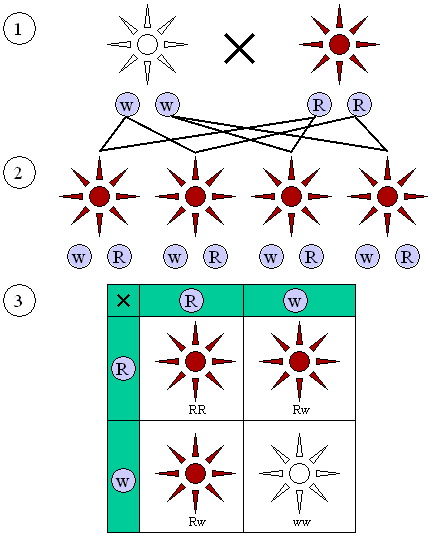
\includegraphics[width=0.5\columnwidth]{../writer/Background/images/Mendelian_inheritance_3_1.png}
	\caption{Image courtesy of Wikimedia Commons}
	\label{fig:back1}
	\end{center}
\end{figure}


Every diploid organism has two alleles that segregate during gamete formation to create diploid offspring that bears just one of the alleles from that parent (i.e. each offspring inherits one allele from their parents). As shown in Figure~\ref{fig:back1}, this has the interesting effect such that two homozygous parents with genotypes \textit{ww} and \textit{RR} respectively will \textit{always} have heterozygous offspring with \textit{wR} genotypes, yet these heterozygous offspring can further mate to reconstitute their parent's genotypes.


\subsubsection{Law of Independent Assortment}

Separate alleles allude to separate traits, and their transmission from parent to offspring are independent of one another. A zygote can end up with any combination of parental alleles, and may end up with genotypes that are entirely different from their parents. Offspring that (by chance) have the same genotypes as any of their parents are called \gls{recombinant}, and offspring with differing genotypes from any of their parents are called \gls{non-recombinant}.

\subsubsection{Law of Dominance}

If the presence of a single form of an allele is enough to produce the phenotype, then that heterozygous allele is said to be \gls{dominant} (as is the case with \textit{wR}, where the \textit{R} trait dominates the w trait). Conversely, if a single form of an allele is \underline{not} enough to produce the phenotype, then that heterozygous allele is said to be \gls{recessive} (as is the case with wR, where the w trait is dominated by the R trait and cannot be expressed).


\subsection{Mendel's Laws Revised}

Though Mendel was ahead of his time in describing genes as allelic traits, he did not take into account that genes from diploid individuals may have more than two alleles (i.e. \gls{multi-allelic}) due to variations within a population.  He also made the erroneous assumption\footnote{One that likely every geneticist makes when first entering the field!} that one allele maps to one trait, where in reality there are numerous \gls{polygenic traits} produced by the interaction of many alleles. 

In relation to his third law, the concept of \gls{codominance} is missed; if the two potential phenotypes within heterozygous alleles are independent of each other and do not conflict, they can both be expressed. Alternately, if the two potential phenotypes within heterozygous alleles are capable of conflicting or interacting with one another, then the phenotype is usually a 'blend' of the two, and said to be of \gls{incomplete dominance} since neither allele is completely dominant over the other.


\subsection{Pedigrees}

\begin{figure}[h]
	\begin{center}
	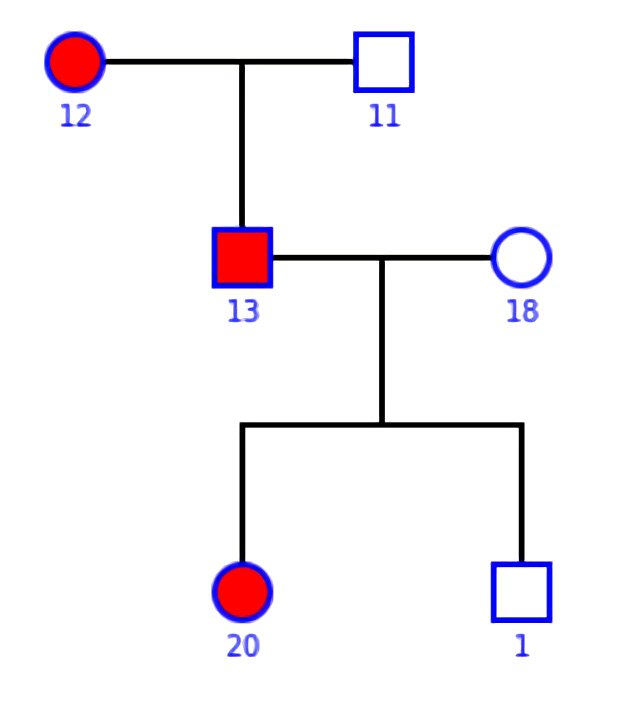
\includegraphics[width=0.5\columnwidth]{../writer/Background/images/simple_pedigree.png}
	\caption{Typical pedigree, with females represented as circles and males as squares. Affectation is represented by a red colour fill.}
	\label{fig:back2pedigree}
	\end{center}
\end{figure}

Individuals from the same family share a \gls{pedigree}, and each individual is grouped into two classes: \gls{founders} and \gls{non-founders}. 
Founders are individuals who contribute unique \gls{founder alleles} to the pedigree, and the non-founders are the individuals who inherit them.
The larger the pedigree the more complex it is to process, with a function that is referred to as the \gls{bit size}.

\begin{equation}
\label{bitsize}
B = 2n -f -g
\end{equation}
where:

\begin{description}
\listitem{n}{number of non-founders}
\listitem{f}{number of founders}
\listitem{g}{number of ungenotyped founder couples}
\end{description}

Inbred pedigrees where related individuals have produced offspring are said to be \gls{consanguineous}.


\subsection{Inheritance Models}

Inheriting a disease allele is not a straightforward process, since the disease may not be visible in every individual who has the allele. For a given individual it is assumed that the disease status is always known\footnote{At least in binary traits which are present at birth.}.  There is an empirical probability that they will present with the disease phenotype, given a set of disease alleles. This is the derived through what is known as a penetrance function:

\begin{equation}
P (D | A) = [0,1]
\end{equation}
where:
\begin{description}
\listitem{D}{Affected or Unaffected}
\listitem{A}{Genotype belonging to {GG,Gg,gg} where G is the disease allele.}
\end{description}


\subsubsection{Autosomal Dominant}

If the disease segregates through an autosomal dominant model, then the disease trait is dominant and the penetrance function is thus:  \(P(D|GG) = P(D|Gg) = 1\), and \(P(D|gg)=0\)
Affected individuals are present at all generations, and because the disease trait lies within the autosomes (chromosomes 1 to 22), affectation is non-gender specific and both sexes have equal probability in inheriting the trait.

\subsubsection{Autosomal Recessive}

Autosomal recessive is a more constrained mode, where instead the disease trait is recessive and the penetrance function is limited to: \(P(D|GG)=1\), and \(P(D|Gg) = P(D|gg) = 0\)

Here, affected individuals appear to skip generations since parents carrying a heterozygous genotype will not present the phenotype, but instead be \gls{carriers} of the disease trait that can be reconstituted as a homozygous disease allele in their offspring. In consanguineous pedigrees, the likelihood of this happening is significantly increased due to the multiple pathways the disease allele can take, with each generation having potentially double the chance of inheriting the disease allele after each subsequent consanguineous pairing.

\subsubsection{X-linked Dominant}

The disease trait rests solely on chromosome X.  Due to males having only one X-chromosome and one Y-chromosome, this simplifies the inheritance pattern such that males can only inherit the single Y-chromosome from their father, and females can only inherit the single  X-chromosome from their father – removing much ambiguity. The male's X-chromosome can still be one of the two maternal X-chromosomes, and likewise the female's maternal X-chromosome can be one of the two as well.  X-linked dominant pedigrees can be identified by a distinct lack of father-to-son transmission, since that would imply that the Y-chromosome is the disease allele. Due to dominant nature of the trait, the penetrance function is identical to that of autosomal dominant.

\subsubsection{X-linked Recessive}

In X-linked recessive diseases, both of the inherited X-chromosomes must contain the disease allele (i.e. be homozygous), with the exception of males who need only copy to express the phenotype since the X-chromosome inherently dominates the Y-chromosome.  Males cannot be carriers in X-linked pedigrees making them \gls{autozygous}.
Typically the pedigree exhibits more affected males than females, with skipped generations where the mother is only a carrier. 
The penetrance function is gender-specific, taking on the same rules for females as autosomal recessive, but differing for males:

\begin{description}
\item[If Female:]{\(P(D|GG)=1, P(D|Gg) = P(D|gg)=0\)}
\item[If Male:]{\(P(D|GG)=N/A,   P(D|Gg)=1, and P(D|gg)=0\)}
\end{description}


\section{Haploblocks}

An individual's genotype is usually acquired in an \gls{unphased} manner, meaning that that genotyping process acquired the alleles present at a locus, but the ordering was unimportant so that the maternal and paternal allele are ambiguous.

A genotype with a known path of inheritance for its alleles is said to be \gls{phased}, and a phased genotype is also known as a \gls{haplotype}.  A haplotype typically spans a single locus similar to an allele, but a haplotype is encapsulated and a restricted to a larger group of haplotypes known as a \gls{haploblock}, which represent the intervals between two recombination events\footnote{Including the recombination that occurs at the start/end of each chromosome}.

These blocks represent the splitting of founder alleles which occurs at every meiosis, effectively halving the founder data within the allele at each generation. 

A founder allele stretching across \textit{m} markers and undergoing \textit{n} meiosis, will have an expected length of \(\frac{m}{n}\) markers over \textit{n} generations.

In Figure~\ref{fig:back_inheritance} the offspring is recombinant at that particular locus due to a crossover in the maternal alleles. Note that at the level of a single marker it is not clear which way a genotype is phased, e.g. the sixth marker where the maternal alleles (2,2) and the paternal alleles (2,2) leave much ambiguity to which particular chromosome the offspring inherited their alleles (2,2).

\begin{figure}[H]
	\begin{center}
	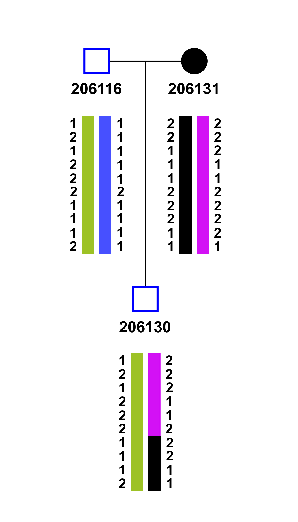
\includegraphics[width=0.5\columnwidth]{../writer/Background/images/simple_inheritance.png}
	\caption2{Four complete haploblocks from two founders inherited by their non-founder offspring. The sixth marker is highlighted due to ambiguous genotypes.}
	\label{fig:back_inheritance}
	\end{center}
\end{figure}


Resolving ambiguous genotypes to specific chromosomes requires providing the genotype with some neighbouring context such that it knows whether it is in a recombination hotspot, or whether it lies within an existing block.  

It is the aim of this thesis to derive methods to explore such problems,  but in order to do so we must first understand how haplotypes are generated through linkage analysis.

\section{Linkage Analysis and Haplotype Generation}

In this chapter we look at the underlying principles that power linkage analysis; the general methodology, as well as the algorithms best suited for generating haplotypes from incomplete genotypes.

\subsection{Theory of Linkage Analysis}

In the previous chapter we discussed how genotypes are mapped to specific markers, and that a disease locus is usually only flanked by the nearest adjacent markers which may or may not be within the same haploblock, and thus may or may not be co-segragated by the disease allele during meiosis.
If a given marker co-segregates with a disease allele over multiple recombination events, then it is safe to assume that they are in close proximity of one another. Such bound loci are said to be \textit{in linkage} with one another, and when one undergoes a meiosis; so does the other.

In linkage analysis, this translates as pinpointing the multiple subsets of markers with the fewest number of crossovers between themselves, such that the the number of meioses in the cases is minimized and the controls are maximized (i.e. which markers/traits are in linkage with one another in affected individuals, but are not in linkage within unaffected individuals).
Classical linkage analysis involves doing this by direct means; counting each crossover event for each marker against every other marker, but the complexity of such a task scales exponentially for large sets and is almost highly impractical.

Modern linkage analysis determines this using statistical means; through the filter of the correct genetic model to establish a correct penetrance function,  the assumption of linkage equilibrium between markers to simplify computation by discounting crossover interference, the lack of monozygotic twins\footnote{Identical genotypes in twins bias the analysis since meioses may not be independent.}, and the known recombination frequencies between markers as well as their ordering. These are then used to establish a likelihood score that rates each marker upon the aforementioned principles such that disease loci can be found by scanning for the highest likelihood.

\subsubsection{Likelihood and LODs}

This likelihood is known as a logarithm of the odds (\gls{LOD}) score, and is a ratio  that compares the likelihood of any two traits being in linkage compared to them not being in linkage. 

\begin{equation}
LOD(\theta) = log_{10} (\frac{L(\hat{\theta})}{L(\theta = 0.5)}
\end{equation}

where:
\begin{itemize}
\listitem{\bf \( \theta = \frac{1}{2}(1 - e^{-2d}) \)}{
The Haldane map function that estimates the recombination frequency given the genetic distance in centiMorgan (as defined in equation~ \ref{eqn:morgan} on page~\pageref{eqn:morgan}).
}
\listitem{\bf \( \theta = 0.5 \)}{
The probability that  two traits segregate independently (are essentially unlinked).
}
\listitem{\bf \( L(\theta)\)}{The joint likelihood}
\end{itemize}

The joint likelihood is main core of what the linkage analysis tries to solve, iterating over all individuals and markers, as defined by:


\begin{equation}
L = \sum_{g1} \dots \sum_{gn} \prod P(Y_i|g_i) \prod_{k,l,m} P(g_m|g_k,g_l)
\end{equation}

\pagebreak
where:
\begin{spacing}{1}
\begin{description}
\listitem{\(g_n=\)}{genotypes of individual \textit{n}}
\listitem{\(Y_n=\)}{phenotype of individual \textit{n}}
\listitem{\(P(Y_i|g_i)=\)}{penetrance probability applied over all individuals. This is the probability of a phenotype given a genotype.}
\listitem{\(P(g_j)=\)}{founder probability applied to founders only. Modelled under Hardy-Weinberg and assumes linkage equilibrium.}
\listitem{\(P(g_m|g_k,g_l)=\)}{transmission probability. Probability of non-founder genotypes (m) given parental genotypes (k and l).}
\end{description}
\end{spacing}

%%% TURN THIS INTO AN NEW COMMAND ENVIRONMENT THAT DOESN'T MESS UP WITH LINE SPACING

There is a narrow window of relevance when dealing with LOD scores, typically any score less than -2 suggests complete lack of linkage and though may seem uninformative, is actually a good indicator of where a disease locus \textit{cannot} be.

A LOD score greater than or equal to 3 is considered to be of great significance for pinpointing a disease locus, but the reasoning for this is mostly historical.

\subsection{Linkage Algorithms}

Though the methodology between algorithms varies somewhat, all work under the same principle of determining a LOD score and generating missing genotypes, though some are more engineered towards resolving phase than others.

\subsubsection{Elston-Stewart}

The very first linkage algorithm first computed upon paper, by performing a task known as peeling upon a \gls{pedigree}.

A connected graph of individuals (as nodes) and relationships (as edges) would be recursively peeled in a depth-first manner, by collapsing LOD score calculations onto members of a pedigree known as \textit{pivots}, who are key to the pedigree such that their removal would create two detached pedigrees. 

At each stage, the algorithm considers a simple nuclear family (mother, father, offspring(s)) and performs a LOD score computation of the offspring inheriting their founder parents genotypes, then flattening the score up a generation into that founder parent.

This eventually resorts in a single node that contains the total LOD summation of the entire pedigree for a given marker.

Over time, programs such as \textbf{Linkage} allowed multiple markers to be considered at the same time and gave rise to \gls{multi-point parametric} linkage analysis that became the standard for subsequent linkage packages.

The algorithm scales linearly with the number of individuals in a pedigree, but exponentially with the number of markers for a multi-point analysis; a severe limiting step in an age where the density of markers were on the increase.

Generating fast and reasonable accurate LOD results became the main aim for a lot of programs, each performing a different approximation upon the LOD score calculations to generate a faster analysis. The program \textbf{Vitesse} was boasted as being able to analyse 8 markers jointly using "fuzzy inheritance".

Since haplotype reconstruction requires precise determination of a missing genotype, the Elston-Stewart algorithm was lacking in this regard.

\subsubsection{Lander-Green}
\subsubsection{Hidden Markov Models and Haplotype Reconstruction}
\subsubsection{Viterbi Algorithm}

\section{Summary}
